% One level of the hybrid builder. Standalone:
%   pdflatex diagram-final-grok.tex
% Copy the PDF to paper/figs/approach-hybrid.pdf.
\documentclass[tikz,border=2pt]{standalone}
\usetikzlibrary{arrows.meta,fit,backgrounds}
\begin{document}
\sffamily
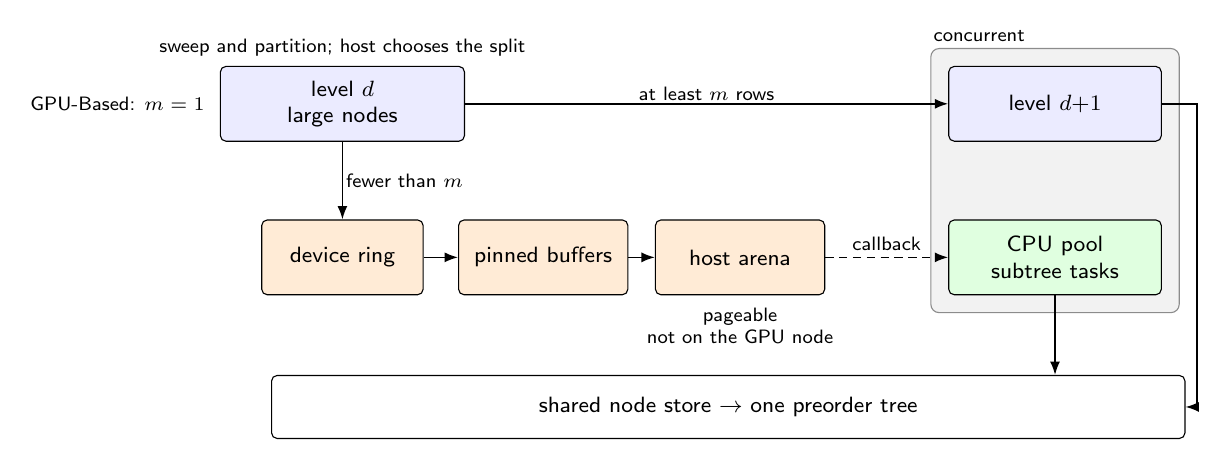
\begin{tikzpicture}[
  box/.style={draw, rounded corners=2pt, align=center, inner sep=3pt,
              font=\footnotesize\sffamily, minimum height=9.5mm},
  gpu/.style={box, fill=blue!8},
  buf/.style={box, fill=orange!16},
  cpu/.style={box, fill=green!12},
  arr/.style={-{Latex[length=1.7mm]}, semithick},
  ctrl/.style={-{Latex[length=1.7mm]}, densely dashed, semithick},
  note/.style={font=\scriptsize\sffamily, align=center, inner sep=1pt}
]

  \node[gpu, minimum width=3.1cm] (level) at (0,0)
    {level \(d\)\\large nodes};
  \node[gpu, minimum width=2.7cm] (next) at (9.05,0)
    {level \(d{+}1\)};
  \node[buf, minimum width=2.05cm] (ring) at (0,-1.95)
    {device ring};
  \node[buf, minimum width=2.15cm] (pin) at (2.55,-1.95)
    {pinned buffers};
  \node[buf, minimum width=2.15cm] (arena) at (5.05,-1.95)
    {host arena};
  \node[cpu, minimum width=2.7cm] (tasks) at (9.05,-1.95)
    {CPU pool\\subtree tasks};
  \node[box, minimum width=11.6cm, minimum height=8mm] (store) at (4.9,-3.85)
    {shared node store \(\rightarrow\) one preorder tree};

  \draw[arr] (level) -- node[note, above] {at least \(m\) rows} (next);
  \draw[arr] (level.south) -- node[note, right] {fewer than \(m\)} (ring.north);
  \draw[arr] (ring) -- (pin);
  \draw[arr] (pin) -- (arena);
  \draw[ctrl] (arena.east) -- (tasks.west)
    node[note, midway, above=1pt] {callback};

  \begin{scope}[on background layer]
    \node[draw=black!45, fill=black!5, rounded corners=3pt,
          fit=(next)(tasks), inner sep=2.2mm] (band) {};
  \end{scope}
  \node[note, anchor=south west] at ([yshift=0.4mm]band.north west) {concurrent};

  % Level d+1 joins the store down the right side, clear of the CPU box.
  \draw[arr] (next.east) -- ++(4.5mm,0) |- (store.east);
  \draw[arr] (tasks.south) -- (tasks.south |- store.north);

  \node[note, anchor=north] at ([yshift=-1.2mm]arena.south)
    {pageable\\not on the GPU node};
  \node[note, anchor=south] at ([yshift=0.8mm]level.north)
    {sweep and partition; host chooses the split};
  \node[note, anchor=east] at ([xshift=-1.5mm]level.west)
    {GPU-Based: \(m=1\)};
\end{tikzpicture}
\end{document}
